\section{Introduksjon}

\subsection{Bakgrunn}
I ett samfunn hvor fler og fler bruker bil som transportmiddel, er det ett stadig økende problem i storbyer en mangel på parkeringsplasser. Det er flere som bor i utkanten og jobber i sentrum og gjerne bruker bilen til og fra jobb. Dette har skapt en stor etterspørsel etter parkering, noe som ikke prioriteres i moderne byutvikling. De plassene som allerede er tilgjengelig er gjerne dyre og ikke alltid tilgjengelig der du trenger dem. Men det finnes også de som eier parkeringsplasser eller områder som det kan være mulig for folk å parkere. Noen har parkeringsplass i forbindelse med boligen de eier, men kanskje ikke har bil. Eller bruker sin egen bil til jobb, og dermed er parkeringsplassen ledig i normal arbeidstid.

Det er vanskelig for privatpersoner å ha en oversikt og håndtere dette på egenhånd. Så det er dermed et ønske om å utvikle en tjeneste hvor brukere, kan leie tilgjengelige parkeringsplasser i perioder. Og leie ut sin egn plass når de ikke trenger den selv.

% I en samfunn hvor flere og flere mennesker har bil, så har det blitt laget flere parkeringsplasser i sentrum. Disse parkeringsplassene er dyre å booke, dermed er det mer ettertraktet å leie parkeringsplasser for en hvis tidsperiode. For vanlige privatpersoner og små firmaer er det vanskelig å håndtere den digitale infrastrukturen som er rundt disse parkeringsplasser som hvor man finner parkeringsplass, hvor man kan legge de til leie og lignende.

% Det er da et ønske å utvikle et felles system hvor de kan håndtere mest mulig av det som angår brukere.I tjenesten skal noen aktører kunne registrere tilgjengelige plasser som kan leies ut, mens sluttbrukere kan se, reservere og betale for parkeringsplassen i den tiden de trenger det.


\subsection{Problemstilling}
Tjenesten skal ha funksjoner som på en enkel måte lar brukere leie andre sine parkeringsplasser. Og leie ut sin egen om de ønsker det. Betaling for leien skal skje igjennom tjenesten.

Det skal også være mulig for brukeren å se en oversikt over de plassene man selv leier ut. Og plasser som tidligere har vært leid.

Ett ønske er at tjenesten skal være tilgjengelig på pc, nettbrett og telefon. Slik at man lett kan bruke tjenesten når man ønsker det.

% Tjenesten skal ha funksjoner som gjør det mulig å leie parkeringsplasser og legge ut parkeringsplasser for andre å leie. Den skal også være brukervennlig slik at de fleste forstår tjenesten. 

%  Den skal også være mulig å se en oversikt over de utleide plassene aktøren har og de leide plassene aktøren leier. 
% Det skal også være mulig å betale for de ulike parkeringsplassene, slik at alt det digitaliserte infrastrukturen er implementert i selve tjenesten. 

% En av problemstillingene vi ønsker er at den skal være mulig å være på både telefon, tablet og datamaskiner, og at den er tilpasset til alle. Og at den ikke bryter noen regler.


\subsection{Mål}

For at tjenesten skal være tilgjengelig på flere plattformer trenger kjernesystemet å være tilgjengelig via internett. Ved å lage en API (\textit{application programming interface}) så kan forskjellig typer brukergrensesnitt kommunisere med systemet på samme måte. Dette uten å måtte tilpasse kjernesystemet til de forskjellige. Det er kjernesystemet som behandler alt av forespørsler, og det er her forretningens logikk håndterer dataflyten til og fra databasen.

\begin{figure}[H]
    \centering
    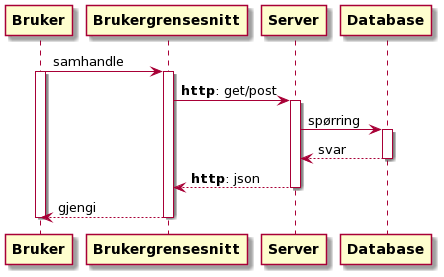
\includegraphics[width=10cm]{bilder/uml/intro_flyt.png}
    \caption{Overordnet oversikt over dataflyt mellom brukergrensesnitt, server og database.}
    \label{fig:lagdeling}
\end{figure}

I denne oppgaven har vi valgt å lage ett forenklet brukergrensesnitt for nettleseren. Men muligheten er mange hvor en slik tjeneste kan passe inn.  Man kan skape mobilapplikasjon eller mulighet for å integrere tjenesten i andre systemer, slik som hotell bookingsider, airbnb eller liknende.

Målet er også å skape brukervennlige funksjoner, som er lette å forstå. Slik at tjenesten skal kunne brukes av voksne i alle aldre, uten spesielt teknisk kunnskap.  Tjenesten skal oppfyller de kravene som raskest gir kunden verdi. I form av en prototype har vi utviklet et «\textit{minste brukbare produkt}» (engelsk: «\textit{minimum viable product (MVP)}»). Som viser kjernefunksjonene i systemet.



For at oppstartsbedriften skal kunne tjene penger på ideen sin. Er det viktig at løsningen vil generer penger, og brukere samtidig. Vi foreslår at brukere som kun leier plass ikke trenger å betale noe for tjenesten. Og for de som ønsker å leie ut, så er de første 6 månedene avgiftsfrie. Etter det vil det påløpe ett gebyr på 20\% av leieinntektene. Dette vil sørge for at brukere som er interessert kan prøve tjenesten kostnadsfritt. Og på den måten skape en brukerbase raskest mulig. Skal du leie ut mer enn 3 plasser, blir du ansett som næringsdrivende. Da vil det bli en løpende månedskostnad på noen hundre kroner.


Videre i denne prosjektdokumentasjonen vil vi beskrive de forskjellige delene av systemet i mer detalj. Og forklare mer om hva og hvordan vi har tenkt at et slik system skal virke. Hvem dens brukere er, vise til tenkte bruker scenarioer, estimere og forklare vår prototype.


% Det er derfor viktig at programvaren har mulighet for å virke både på mobil, gjerne via en applikasjon og i nettleseren. Begge disse plattformene bruker internett for å kommunisere, og vil da være lurt at selve systemet som håndterer alt av databaser og buisness-logikk kan kommuniseres med via en API (\textit{application programming interface}). Dette muliggjør at systemet kan utvides med forskjellige typer brukergrensesnitt i fremtiden. Uten å måtte endre på kjernen i systemet. I denne oppgaven vil vi bruke et forenklet brukergrensesnitt for nettleseren. Men muligheten er mange. Man kan skape mobilapplikasjon eller mulighet for å integrere tjenesten i andre systemer, slik som hotell booking sider, air-bnb eller liknende.
% Målet er også å ha brukervennlige funksjoner, som er lett å forstå. Og at tjenesten oppfyller de kravene vi setter som MVP (\textit{minimum viable product}) som gir kundene verdi.


%  Videre i denne prosjektdokumentasjonen vil vi beskrive de forskjellige delene av systemet i mer detalj. Og forklare mer hva og hvordan vi har tenkt at et slik system skal virke, hvem dens brukere er, vise til tenkte bruker scenarioer, estimere og forklare vår prototype.